%% 
%% This is file ejmcls.ltx - generated with MakeDist v1.0, by M. Reed 
%% 
 
\documentclass{article}

\usepackage[utf8]{inputenc}
\usepackage{lmodern}


\usepackage{geometry}                		% See geometry.pdf to learn the layout options. There are lots.
\geometry{letterpaper}                   		% ... or a4paper or a5paper or ... 
%\geometry{landscape}                		% Activate for for rotated page geometry
%\usepackage[parfill]{parskip}    		% Activate to begin subsubsections with an empty line rather than an indent
\usepackage{graphicx}				% Use pdf, png, jpg, or eps§ with pdflatex; use eps in DVI mode
								% TeX will automatically convert eps --> pdf in pdflatex		
\usepackage{fancyhdr}
\usepackage{amssymb}
\usepackage{dsfont}
\usepackage{amsmath}
\usepackage{pgfplots}
\usepackage{tikz}
\usepackage{enumerate}
\usepackage{quoting}
\usepackage{amsthm}

\usetikzlibrary{patterns}
\usetikzlibrary{decorations.text}
\usetikzlibrary{decorations.pathmorphing}

\usepackage{caption}
\usepackage{subfig}
%\usepackage{subcaption}
\usepackage{geometry}
%\geometry{top=2cm, bottom=2cm, left=2cm, right=2cm}
\geometry{margin=2cm}

\author{Gil-Arnaud Coche}
%\date{}							% Activate to display a given date or no date


\tikzset{
  pics/carc/.style args={#1:#2:#3}{
    code={
      \draw[pic actions] (#1:#3) arc(#1:#2:#3);
    }
  }
}



\numberwithin{equation}{section}

\setlength{\parindent}{0in}

\definecolor{awesomePurple}{rgb}{0.55, 0.42, 1}

\begin{document}

\newtheorem{hyp}{Hypothese}
\newtheorem*{hyp*}{Hypothese}

\pgfdeclarepatternformonly[/tikz/radius,\thickness,\size]{rings}
{\pgfpoint{-0.5*\size}{-0.5*\size}}
{\pgfpoint{0.5*\size}{0.5*\size}}
{\pgfpoint{\size}{\size}}
{
  \pgfsetlinewidth{\thickness}
  \pgfpathcircle\pgfpointorigin{\pgfkeysvalueof{/tikz/radius}}
  \pgfusepath{stroke}
}
\newdimen\thickness
\tikzset{
  radius/.initial=4pt,
  size/.store in=\size, size=20pt,
  thickness/.code={\thickness=#1},
  thickness=0.75pt
}

\newcommand{\W}{\mathcal{W}}
\newcommand{\G}{\mathcal{G}}
\newcommand{\N}{\mathcal{N}}
\newcommand{\diff}{\textnormal{d}}

\title{Allocation optimale avec consommation du capital.}

\author{Gil-Arnaud Coche}
\maketitle

Dans cette note, on va chercher à comprendre les points essentiels d'une allocation de richesse entre un actif risqué et un actif sans risque, sachant que l'investisseur consomme son capital sur la période. On s'intéresse au cas simple mais instructif d'un investissement de $k = 0$ à $k = 1$.\\

\section{Le modèle}

Mettons-nous dans la peau d'un petit porteur qui a à sa disposition un capital $\W_0$ à l'instant 0. On va essayer de comprendre comment ce petit porteur pourrait répartir ce capital jusqu'à l'instant 1 entre 
\begin{itemize}
\item un actif risqué de rendement 
$$
\mu = m + \sigma\epsilon
$$
où $\epsilon$ est une loi normale centrée et réduite;
\item un actif sans risque de rendement $r$;
\end{itemize}
sachant qu'il souhaite consommer $c_0$ et $c_1$ de ce capital en 0 et 1 respectivement.

\begin{figure}[h!]
\centering
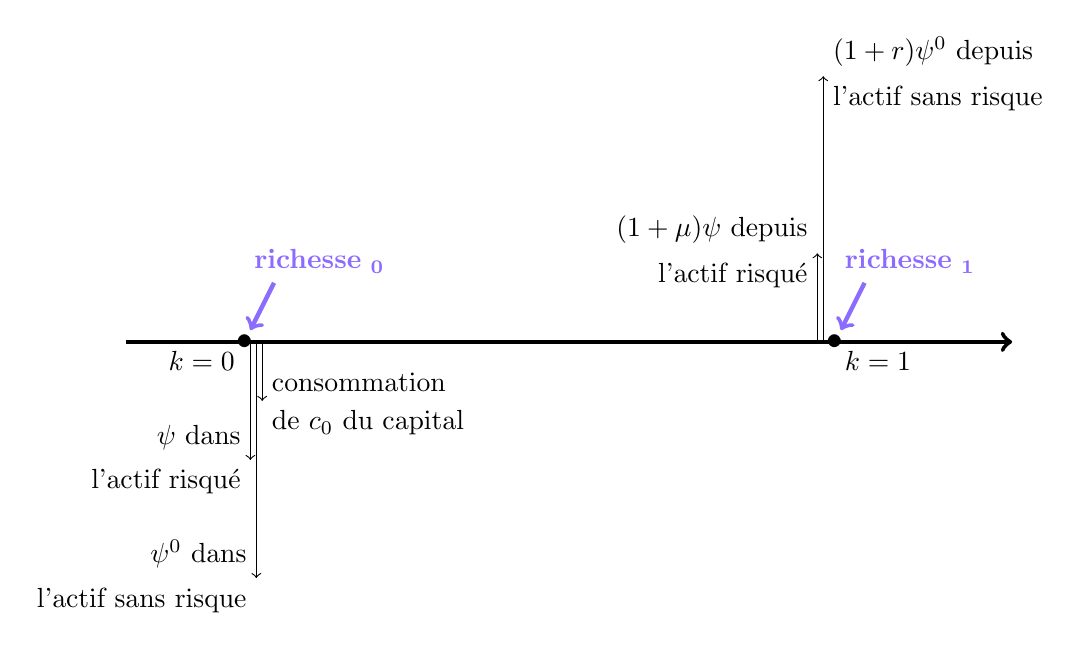
\begin{tikzpicture}[scale = .75]
\draw[->, ultra thick] (-2, 0) -- (13, 0);

\node at (0, 0) {\large $\bullet$};
\node at (0, 0) [below left] {$k = 0$};
\node at (0, 1) [above right] {\color{awesomePurple}\textbf {richesse} $\boldsymbol {\W_{0}}$};
\draw [->, ultra thick, awesomePurple] (.5, 1) -- (0.1, .2);

\node at (10, 0) {\large$\bullet$};
\node at (10, 0) [below right] {$k = 1$};
\node at (10, 1) [above right] {\color{awesomePurple}\textbf {richesse} $\boldsymbol {\W_{1}}$};
\draw [->, ultra thick, awesomePurple] (10.5, 1) -- (10.1, .2);

\draw[->] (0.1, 0) -- (0.1, - 2);
\node at (0.1, -2) [above left] {$\psi$ dans};
\node at (0.1, -2) [below left] {l'actif risqué};

\draw[->] (.2, 0) -- (.2, - 4);
\node at (.2, -4) [above left] {$\psi^0$ dans};
\node at (.2, -4) [below left] {l'actif sans risque};

\draw[->] (.3, 0) -- (.3, - 1);
\node at (.3, -1) [above right] {consommation};
\node at (.3, -1) [below right] {de $c_0$ du capital};


\draw[->] (9.7, 0) -- (9.7, 1.5);
\node at (9.7, 1.5) [above left] {$(1 + \mu)\psi$ depuis};
\node at (9.7, 1.5) [below left] {l'actif risqué};

\draw[->] (9.8, 0) -- (9.8, 4.5);
\node at (9.8, 4.5) [above right] {$(1 + r)\psi^0$ depuis};
\node at (9.8, 4.5) [below right] {l'actif sans risque};

\end{tikzpicture}
\caption{Les flux de richesse entre deux instant de gestion $k = 0$ et $k = 1$.}
\label{fig:flux-de-richesse}
\end{figure}

D'après la figure \ref{fig:flux-de-richesse}, le petit porteur place en l'instant $k = 0$
\begin{itemize}
\item une valeur $\psi$ dans l'actif risqué;
\item une valeur $\psi^0$ dans l'actif sans risque.
\end{itemize}
Il consomme également $c_0$, de sorte que sa initiale richesse $\W_0$ peut s'exprimer comme la somme de $\psi$, $\psi^0$ et de $c_0$
\begin{equation}\label{eq:conservation-zéro}
\W_0 = \psi + \psi^0 + c_0.
\end{equation}
En l'instant $k = 1$, il reçoit 
\begin{itemize}
\item une valeur $(1 + \mu)\psi$ de son placement risqué;
\item une valeur $(1 + r)\psi^0$ de son placement sans risque.
\end{itemize}
et il se verse l'intégralité de ce qu'il a. Mathématiquement nous avons donc les égalités
$$
c_ 1 = \W_1 = (1 + \mu)\psi + (1 + r)\psi^0.
$$
En prenant en compte la relation \eqref{eq:conservation-zéro} dans l'expression ci-dessus, on obtient
\begin{equation}
c_1 = (\mu - r)\psi + (1 + r)\left(\W_0 - c_0\right).
\end{equation}

Le porteur percevra donc les flux actualisés suivants
\begin{equation}
\tilde\G = c_0 + \frac{c_1}{1 + r} = \W_0 + \frac{m - r + \sigma\epsilon}{1 + r}\psi
\end{equation}

\section{La stratégie d'investissement du petit porteur, solution d'un problème d'optimisation}

\subsection{Benchmark linéaire}

Pour se benchmarker, le petit porteur part du principe que sans stratégie d'investissement, il pourrait tout simplement placer $\psi^0 = \W_0/2$ en l'actif sans risqué et percevoir $c_0 = \W_0/2$ à l'instant initial. Cela lui assurerait d'obtenir $(1 + r)W_0/2$ en l'instant $k = 1$ et ne pas trop subir les affres de l'inflation.\\

\subsection{Son objectif d'investissement.}

Il souhaite à présent bénéficier d'une position en l'actif risqué pour essayer d'augmenter ses rendements. Il cherche donc à chercher le couple $(c_0, \psi)$ qui lui permettra d'assurer une rente actualisée supérieure à $\W_0$.\\

Mathématiquement, on considère que ce porteur veut maximiser son espérance de gains actualisés par rapport à sa richesse initiale $\W_0$.
\begin{equation}
\max_{c_0, \psi} \frac{m - r}{1 + r}\psi
\end{equation}

L'équation ci-dessus étant linéaire en $\psi$, tout optimisation numérique ira chercher la plus grande valeur possible pour $\psi$. En l'absence de contraintes, l'optimisation n'aurait pas donc pas de solutions. C'est justement la nature des contraintes qui va déterminer la stratégie optimale.

\subsection{Ses contraintes d'investissement.}

Néanmoins, il ne veut pas non plus prendre des risques inconsidérés. Il veut donc maîtriser au maximum les possibilités de pertes. Sa mesure du risque sera la probabilité que son investissement lui rapporte en $k = 1$ moins que $(1 + r)\W_0/2$, ce qu'il aurait avec la stratégie sans risque.\\

\textbf{\color{awesomePurple}Ce choix de contrainte est cohérent avec sa démarche de prise de risque: pourquoi investir dans l'incertain si la probabilité de faire moins que son benchmark naïf et certain lui semble trop élevée?}\\

Quantitativement, il se fixe un niveau $\alpha$ de probabilité de perte qu'il juge maximal: il rejettera toute stratégie qui ne lui assurerait pas un probabilité $1 - \alpha$ de faire mieux que son benchmark.\\

Mathématiquement cela se traduit par l'inégalité
$$
\mathds P\left( \left(m - r + \sigma\epsilon\right)\psi \leq \left(1 + r\right)\left( c_0 - \frac{\W_0}{2} \right) \right) \leq \alpha.
$$
Pour y voir plus claire, un peu de développements sont nécessaires. En utilisant l'inverse de la focntion de répartition de la loi normale $\N(x) = \mathds P\left(\epsilon\leq x\right)$, on arrive à
\begin{equation}\label{eq:risk-ineq}
\frac{1+r}{\sigma\psi}\left( c_0 - \frac{\W_0}{2} \right) \leq \frac{m - r}{\sigma} - \N^{-1}\left( 1 - \alpha\right).
\end{equation}

Dans l'expression ci-dessus, on voit apparaître le ratio de sharpe $$s = \frac{m - r}{\sigma}$$ et un ratio de Sharpe limite $$s_\alpha = \N^{-1}\left( 1 - \alpha\right)$$ qui n'est autre que le quantile de niveau $1 - \alpha$ de la distribution de $\epsilon$ (qui est ici gaussienne centrée réduite). Deux cas de figure vont donc se présenter. Avant de les développer, rappelons que l'on a en toute circonstance $0\leq \psi\leq \W_0 - c_0$.

\begin{figure}[h!]
\centering
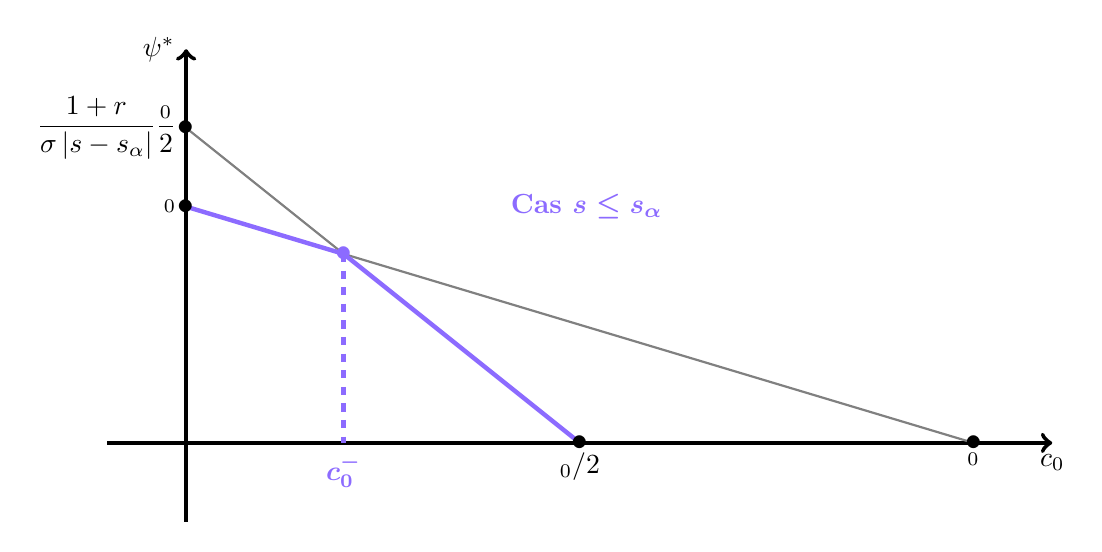
\begin{tikzpicture}

\draw [->, ultra thick] (-1, 0) -- (11, 0) node [below] {$c_0$};
\draw [->, ultra thick] (0, -1) -- (0, 5) node [left] {$\psi^*$};

\draw [thick, gray] (0, 3) -- (10, 0);
\draw [thick, gray] (0, 4) -- (5, 0);

\draw [ultra thick, awesomePurple] (0, 3) -- (2, 2.4);
\draw [ultra thick, awesomePurple] (2, 2.4) -- (5, 0);

\node at (2, 2.4) {\color{awesomePurple}\large$\bullet$};
\draw [ultra thick, awesomePurple, dashed] (2, 2.4) -- (2, 0) node[below]{\color{awesomePurple}$\boldsymbol{c^-_0}$};

\node at (5, 0) {\large$\bullet$};
\node at (5, 0) [below] {$\W_0/2$};

\node at (10, 0) {\large$\bullet$};
\node at (10, 0) [below] {$\W_0$};

\node at (0, 3) {\large$\bullet$};
\node at (0, 3) [left] {$\W_0$};

\node at (0, 4) {\large$\bullet$};
\node at (0, 4) [left] {$\displaystyle{\frac{1+r}{\sigma\left|s - s_\alpha\right|}\frac{\W_0}{2}}$};

\node at (4, 3) [right] {\textbf{\color{awesomePurple}Cas $\boldsymbol{s\leq s_\alpha}$}};

\end{tikzpicture}

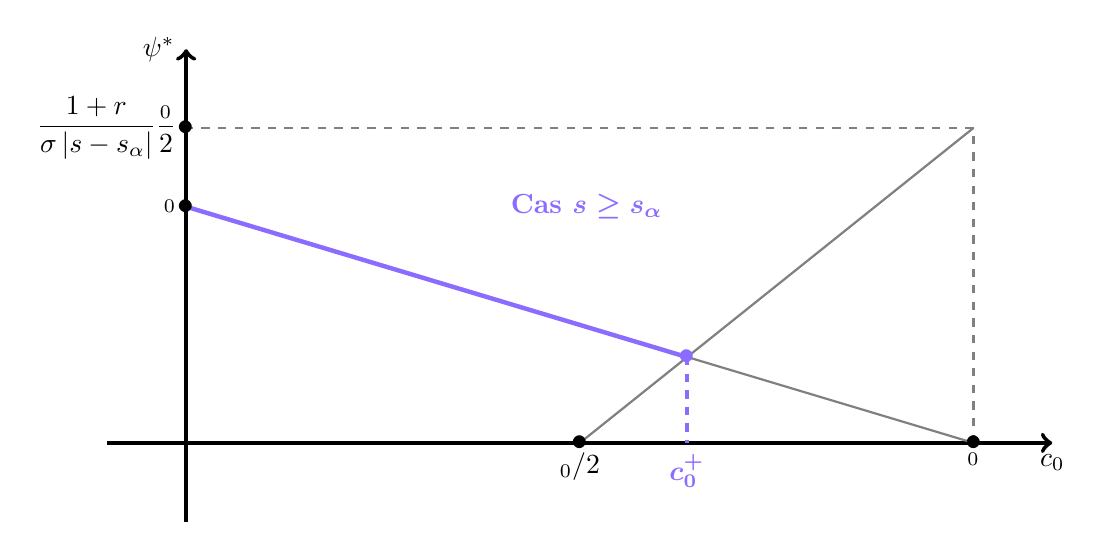
\begin{tikzpicture}

\draw [->, ultra thick] (-1, 0) -- (11, 0) node [below] {$c_0$};
\draw [->, ultra thick] (0, -1) -- (0, 5) node [left] {$\psi^*$};

\draw [thick, gray] (0, 3) -- (10, 0);
\draw [thick, gray] (10, 4) -- (5, 0);
\draw [thick, gray, dashed] (10, 4) -- (0, 4);
\draw [thick, gray, dashed] (10, 0) -- (10, 4);

\draw [ultra thick, awesomePurple] (0, 3) -- (6.36, 1.09);

\node at (6.36, 1.09) {\color{awesomePurple}\large$\bullet$};
\draw [ultra thick, awesomePurple, dashed] (6.36, 1.09) -- (6.36, 0) node[below]{\color{awesomePurple}$\boldsymbol{c^+_0}$};

\node at (5, 0) {\large$\bullet$};
\node at (5, 0) [below] {$\W_0/2$};

\node at (10, 0) {\large$\bullet$};
\node at (10, 0) [below] {$\W_0$};

\node at (0, 3) {\large$\bullet$};
\node at (0, 3) [left] {$\W_0$};

\node at (0, 4) {\large$\bullet$};
\node at (0, 4) [left] {$\displaystyle{\frac{1+r}{\sigma\left|s - s_\alpha\right|}\frac{\W_0}{2}}$};

\node at (4, 3) [right] {\textbf{\color{awesomePurple}Cas $\boldsymbol{s\geq s_\alpha}$}};

\end{tikzpicture}
\caption{L'allocation optimale en actif risqué comme fonction de la consommation $c_0$}
\label{fig:allocation-optim}
\end{figure}

\begin{itemize}
\item\textbf{Cas $\boldsymbol{s\leq s_\alpha}$: l'actif ne performe pas assez pour l'investisseur}

L'inégalité de l'équation \eqref{eq:risk-ineq} devient 
$$
\frac{1+r}{\sigma\left(s_\alpha - s\right)}\left( \frac{\W_0}{2} - c_0 \right) \geq \psi
$$
ce qui donne la condition générale pour la satisfaction des attentes en risques
\begin{equation}
0\leq\psi\leq \min\left( \frac{1+r}{\sigma\left(s_\alpha - s\right)}\left( \frac{\W_0}{2} - c_0 \right), \W_0 - c_0 \right)
\end{equation}

\item\textbf{Cas $s\geq s_\alpha$: l'actif a une performance intéressante pour l'investisseur} 

L'inégalité de l'équation \eqref{eq:risk-ineq} devient cette fois
$$
\frac{1+r}{\sigma\left(s - s_\alpha\right)}\left( c_0  - \frac{\W_0}{2}\right) \leq \psi
$$
et l'on conclut donc que la contrainte sur les risques sera satisfaite à condition que
\begin{equation}\label{eq:cond2}
\frac{1+r}{\sigma\left(s - s_\alpha\right)}\left( c_0  - \frac{\W_0}{2}\right) \leq \psi\leq \W_0 - c_0.
\end{equation}
\end{itemize}

Comme évoqué à la section précédente, la nature linéaire en $\psi$ de la fonction objectif implique que l'on sature les les bornes supérieures dans les inégalités précédentes. On peut alors tracer l'allocation optimale $\psi^*$ en fonction de la consommation $c_0$ (figure \ref{fig:allocation-optim}).\\

\textbf{\color{awesomePurple}Pour des ratios de sharpes plus petit que le niveau exigé par l'aversion au risque du porteur, il est inutile d'investir dans l'actif risqué si l'on consomme $c_0 = \W_0/2$. Ce qui confirme que l'on peut difficilement battre le marché avec cette stratégie. En revanche, si l'on est patient et que l'on consomme moins, on peut s'attendre à un coupon plus important en période 1 et au global, pourvu que $m>r$, on peut espérer faire un gain total actualisé plus important que $\W_0$ avec une probabilité $\pi$ égale à
\begin{equation}
\pi = \N\left( -s \right)
\end{equation}
Seule la patience permet de créer du levier grâce à une prise de risque maîtrisée.}\\

\textbf{\color{awesomePurple}Pour des ratios de sharpe plus important, il est possible de consommer jusqu'à 
\begin{equation}
c^+_0 = \frac{1 + r + 2\sigma\left( s - s_\alpha \right)}{1 + r + \sigma\left( s - s_\alpha \right)}\frac{W_0}{2}> \frac{W_0}{2}
\end{equation}
comme indiqué par le schéma du bas sur la figure \ref{fig:allocation-optim}. La valeur $c_0^+$ est facilement obtenue en égalisant les bornes de l'inégalité \eqref{eq:cond2}. Si l'on s'intéresse aux ordres de grandeur, on se rend vite compte que cette situation est en fait plutôt rarissime. Pour un niveau $\alpha = 5\%$, il faudrait que l'actif risqué ait un ratio de sharpe de plus de 1.96...}\\


\end{document}